%%%%%%%%%%%%%%%%%%%%%%%%%%%%%%%%%%%%%%%%%
% Short Sectioned Assignment
% LaTeX Template
% Version 1.0 (5/5/12)
%
% This template has been downloaded from:
% http://www.LaTeXTemplates.com
%
% Original author:
% Frits Wenneker (http://www.howtotex.com)
%
% License:
% CC BY-NC-SA 3.0 (http://creativecommons.org/licenses/by-nc-sa/3.0/)
%
%%%%%%%%%%%%%%%%%%%%%%%%%%%%%%%%%%%%%%%%%

%----------------------------------------------------------------------------------------
%	PACKAGES AND OTHER DOCUMENT CONFIGURATIONS
%----------------------------------------------------------------------------------------

\documentclass{article}
\usepackage[utf8]{inputenc}
\usepackage[T1]{fontenc}
\usepackage[slovak,english]{babel}
\newcommand\sktxt[1]{\foreignlanguage{slovak}{#1}}
% English language/hyphenation
\usepackage{amsmath,amsfonts,amsthm} % Math packages
\usepackage{tikz}
\usetikzlibrary{arrows}
\usepackage{multirow}
\usepackage{cases}
\setlength{\headheight}{11pt} % Customize the height of the header
\usepackage{hyperref}
\usepackage[top=2cm, bottom=2cm, right=2cm, left=2cm]{geometry}
\hypersetup{
colorlinks=true,
linkcolor=blue,
filecolor=magenta,
urlcolor=cyan,
}
\numberwithin{equation}{section} % Number equations within sections (i.e. 1.1, 1.2, 2.1, 2.2 instead of 1, 2, 3, 4)
%\numberwithin{figure}{section} % Number figures within sections (i.e. 1.1, 1.2, 2.1, 2.2 instead of 1, 2, 3, 4)
%\numberwithin{table}{section} % Number tables within sections (i.e. 1.1, 1.2, 2.1, 2.2 instead of 1, 2, 3, 4)
\usepackage{xcolor,colortbl}
\definecolor{yellow}{rgb}{0.7,0.7,0}
\definecolor{red}{rgb}{1,0,0}

\title{ Neurónové siete}

\author{Peter Kovács, Marián Margeta, Jakub Pospíchal, Jozef Brandys}
\date{ }
 
\begin{document}

\maketitle
\tableofcontents
\newpage
\section{Dopredné modely. Otázky 1 až 7. }
\subsection{Stručná história konekcionizmu, vlastnosti biologického neurónu, model neurónu s prahovou logikou,
implementácia Booleových funkcií. Paradigmy učenia a typy úloh pre NS.}
Stručná história konekcionizmu sa začína v 40tych rokoch v psychologii a filozofii. McCullogh a Pitts vymyslia neuron s aktivacnym prahom. Neskor v 60. až 70. rokoch sa k ich nápadu vyjadrý Minsky, zrozumitelnejšie to popíše a dá to do kontextu s teóriou formálnych jazykov a automatov. V 90. rokoch prichádzajú na výslnie viacvrstvové generatívne modely a od roku 2000 prichádza druhá renesancia - deep learning, rekurentné a konvolučné neurónové sieťe a tiež siete s echo stavmi.
\\\\
Nervová bunka sa skladá z tela a niekoľkých výbežkov. Tieto možno rozdeliť na dva typy: dendrity, ktoré predstavujú z informatického hľadiska vstupnú časť (predovšetkým na ne prechádza vzruch z iných buniek) a jeden axón, po ktorom sa vzruch šíri k iným bunkám.[Uvod do teórie neurónových sietí.]
\\\\
Neurón s prahovou logikou vyzerá nasledovne, \\
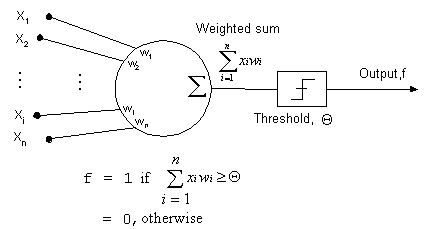
\includegraphics[width=12cm]{imgs/threshold_neuron}\\
v prípade, že by sme pomocou neho chceli implementovať booleovské funkcie, napríklad logický AND jednoducho pre každú premennú použijeme jeden vstup a threshold bude rovný počtu premenných. V prípade OR by stačilo aby threshold bol 1. Ešte by bolo vhodné podotknúť, že každá booleovská funkcia môže byť simulovaná pomocou dvojvrstvovej NN s logickými jednotkami.
\\\\
Medzi paradigmy učenia v neurónových sietiach patrí určite učenie s učiteľom a učenie bez učiteľa. Ako príklad si uveďme cenu domov v Bratislave. Vstupom sú dáta typu rozloha/cena/počet izieb a výstupom cena. V prípade učenia s učiteľom máme dostupnú cenu ktorú chceme predikovať. V prípade učenia bez učiteľa máme k dispozícii iba prvé tri vstupy a na základe nich môžeme byty zhlukovať do kategórií veľký/malý etc. Poslednou paradigmou učenia je učenie posilnovaním, ktoré funguje na základe nejakej funkcie odmeny. Po každej akcii sa posunieme do nového stavu a prostredie nám poskytne informáciu či to čo sme spravili je správne alebo nie.
\\\\
V dnešnej dobe sa neurónové siete používajú na kadečo významné úspechy dosiahli v oblasti spracovania obrazu(konvolučné siete), spracovaní prirodzeného jazyka, zvuku alebo iných sekvenčných dát(rekurentné)...

\subsection{Binárny perceptrón: pojem učenia s učiteľom, učiace pravidlo, algoritmus trénovania, deliaca nadrovina, klasifikácia vzorov, lineárna separovateľnosť, náčrt dôkazu konvergencie, definícia a príklad.}
Binarny perceptron === dáva nám output 1/0 [??]\\
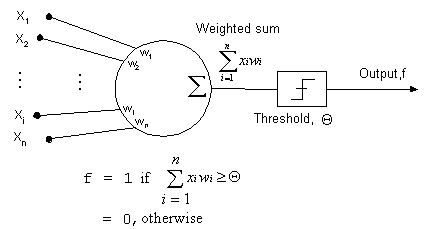
\includegraphics[width=12cm]{imgs/threshold_neuron}\\
Učiace pravidlo updatuje perceptrón na základe toho aký výstup nám vypluje a aký bol požadovaný výstup. 
$$ w_j(t+1) = w_j + \alpha (d-y)x_j $$
kde $w_j$ je váha $j$-teho vstupu $\alpha$ je rýchlosť učenia, $d$ je očakývaný výstup, $y$ je výstup perceptrónu a $x_j$ je $j$-ty vstup.
\\\\
Algoritmus trénovania je nasledovný:
\begin{enumerate}
\item Zvoľ vstup x a vypočítaj výstup y.
\item Spočítaj chybovú funkciu $e(t) = 1/2(d-y)^2$ a pripočítaj k celkovej chybe $E := E + e(t)$.
\item uprav všetky váhy na základe učiaceho pravidla (ak e(t) > 0),
\item ak som použil všetky trénovacie vstupy goto 5. inak goto 1.
\item ak $E = 0$ (setky patterny su spravne zaklasifikovane) skonči inak poprehadzuj vstup $ E := 0 $ a začni od 1.
\end{enumerate}
To čo vlastne perceptrón spraví je, že rozdelí(klasifikuje) vstupy do dvoch tried, tie ktoré ho aktivujú a tie ktoré nie. Vo všeobecnosti perceptrón len hľadá nejakú deliacu nadrovinu, ktorú vieme zapísať v tvare $\sum_{i=1}^n w_ix_i = \theta$.
\\\\
V roku 1962 Rosenblatt sformuloval vetu: Nech triedy A a B sú lineárne separoveteľne(existuje nadrovina, ktorá správne oddeli jednu triedu od druhej) potom perceptrón konverguje, tj. nájde deliacu nadrovinu, ktorá rozdelí tieto dáta do dvoch množín.
\\\\
Dôkaz:
% pouzite video na https://www.youtube.com/watch?v=-j8wi1OLO4Y

Vezmime si dve lineárne separovateľné triedy $C_1$ a $C_2$. Váhy predstavuje matica $w$. Rovnica priamky oddeľujúcej triedy je $\overrightarrow{w}^T\cdot \overrightarrow{x} = 0$.

Máme nejakú trénovaciu množinu $H_1$ ($H_2$), ktorej prvky patria do triedy $C_1$ ($C_2$).

Platí:
$$\overrightarrow{w}^T \cdot \overrightarrow{x} > 0, \qquad \overrightarrow{x} \in C_1$$
$$\overrightarrow{w}^T \cdot \overrightarrow{x} \leq 0, \qquad \overrightarrow{x} \in C_2$$

Teraz, weight update algoritmus bude fungovať:
\begin{enumerate}
\item Take $\overrightarrow{x}(n)$
$$\overrightarrow{w}(n+1) = \overrightarrow{w}(n),\qquad ak~ \overrightarrow{w}^T(n)\cdot\overrightarrow{x}(n) > 0 ~\land~ \overrightarrow{x}(n) \in C_1$$
$$\overrightarrow{w}(n+1) = \overrightarrow{w}(n),\qquad ak~ \overrightarrow{w}^T(n)\cdot\overrightarrow{x}(n) \leq 0 ~\land~ \overrightarrow{x}(n) \in C_2$$
\item 
$$\overrightarrow{w}(n+1) = \overrightarrow{w}(n) - \alpha\overrightarrow{x}(n),\qquad ak~ \overrightarrow{w}^T(n)\cdot\overrightarrow{x}(n) > 0 ~\land~ \overrightarrow{x}(n) \in C_2$$
$$\overrightarrow{w}(n+1) = \overrightarrow{w}(n) + \alpha\overrightarrow{x}(n),\qquad ak~ \overrightarrow{w}^T(n)\cdot\overrightarrow{x}(n) \leq 0 ~\land~ \overrightarrow{x}(n) \in C_1$$
\end{enumerate}

Proof: 

Assumptions:
\begin{itemize}
\item Lineárna separovateľnosť
\item $\overrightarrow{w}(0) = \overrightarrow{0}$
\item $\alpha = 1$
\end{itemize}

Vezmime si $\overrightarrow{x}(n)$ pre $n = 1,2,3 \ldots$ tak, že $\overrightarrow{x}(n) \in H_1$ a zároveň všetky odpredikujeme zle. Teda platí:
$$\overrightarrow{w}(n+1) = \overrightarrow{w}(n) + \overrightarrow{x}(n)$$
\begin{equation}\label{eq:1}
\overrightarrow{w}(n+1) = \overrightarrow{x}(1) + \overrightarrow{x}(2) + \ldots + \overrightarrow{x}(n)
\end{equation}

Z toho že $C_1$ a $C_2$ sú lineárne separovateľné vyplýva, že existuje riešenie $w_0$, pre ktoré platí:
$$\overrightarrow{w}_0^T \cdot \overrightarrow{x}(n) > 0, \qquad for~ \overrightarrow{x}(1), \overrightarrow{x}(2), \ldots \overrightarrow{x}(n) \in H_1$$
Z toho si vyvodíme $a$:
$$a = \min_{\overrightarrow{x}(n) \in H_1}{\overrightarrow{w}_0^T \cdot\overrightarrow{x}(n)} $$
Prenásobme rovnicu \ref{eq:1} zľava $\overrightarrow{w}_0^T$:
$$\overrightarrow{w}_0^T\overrightarrow{w}(n+1) = \overrightarrow{w}^T_0\cdot\overrightarrow{x}(1) + \ldots \overrightarrow{w}_0^T\cdot\overrightarrow{x}(n)$$
\begin{equation}\label{eq:2}
\overrightarrow{w}_0^T\overrightarrow{w}(n+1) \geq n\cdot a
\end{equation}
Napíšme si teraz Cauchy--Schwarzovu nerovnosť:
$$\lVert \overrightarrow{w}_0 \rVert^2 \lVert \overrightarrow{w}(n+1) \rVert ^2 \geq [\overrightarrow{w}_0^T \overrightarrow{w}(n+1)]^2$$
Použitím \ref{eq:2} dostávame:
$$\lVert \overrightarrow{w}_0 \rVert^2 \lVert \overrightarrow{w}(n+1) \rVert ^2 \geq n^2a^2$$
Následne upravíme na:
\begin{equation}\label{eq:3}
\lVert \overrightarrow{w}(n+1) \rVert ^2 \geq \frac{n^2a^2}{\lVert \overrightarrow{w}_0 \rVert^2}
\end{equation}

Vďaka \ref{eq:3} máme dolné ohraničenie, ale ešte potrebujeme horné, vezmime si teda alternatívny prístup:
$$\overrightarrow{w}(k+1) = \overrightarrow{w}(k) + \overrightarrow{x}(k), \qquad for~ k = 1, 2, \ldots n ~\land~ \overrightarrow{x}(k) \in H_1$$
Squared euclidean norm of:
$$\lVert \overrightarrow{w}(k+1)\rVert^2 = \lVert \overrightarrow{w}(k)\rVert^2 + \lVert \overrightarrow{x}(k)\rVert^2 + 2\overrightarrow{w}^T(k)\cdot\overrightarrow{x}(k)$$
Perceptron je zle natrénovaný pred $k = 1,2, \ldots n$ a keďže prvky sú z $H_1$, tak platí $\overrightarrow{w}^T(k)\cdot\overrightarrow{x}(k) < 0$. Potom:
$$\lVert \overrightarrow{w}(k+1) \rVert^2 \leq \lVert \overrightarrow{w}(k) \rVert^2 + \lVert \overrightarrow{x}(k) \rVert^2$$
$$\lVert \overrightarrow{w}(k+1) \rVert^2 - \lVert \overrightarrow{w}(k) \rVert^2\leq \lVert \overrightarrow{x}(k) \rVert^2$$
Teda:
$$\lVert \overrightarrow{w}(n+1) \rVert^2 \leq \sum_{k=1}^{n} \lVert \overrightarrow{x}(k)\rVert^2 $$
Vyjadríme si $b$:
$$b = \max_{\overrightarrow{x}(k) \in H_1}{\lVert \overrightarrow{x}(k) \rVert ^2}$$
Potom platí:
\begin{equation}\label{eq:4}
\lVert \overrightarrow{w}(n+1) \rVert^2 \leq nb
\end{equation}
Z rovnice \ref{eq:4} máme horné ohraničenie.

Teraz už len definujeme $n_{max}$, kedy aj pre rovnice \ref{eq:3} aj \ref{eq:4} nastáva rovnosť.
$$ \frac{n_{max}^2a^2}{\lVert \overrightarrow{w}_0 \rVert^2} = n_{max}b$$
$$n_{max} = \frac{b\cdot\lVert\overrightarrow{w}_0\rVert^2}{a^2}$$

Juchú. \qed

Pre lepšie pochopenie odporúčam video na youtube, napr.: \url{https://www.youtube.com/watch?v=-j8wi1OLO4Y}.



\subsection{Spojitý perceptrón: Rôzne aktivačné funkcie perceptrónu, chybová funkcia a spôsob jej minimalizácie, učiace pravidlo, algoritmus trénovania perceptrónu. Súvis s Bayesovským klasifikátorom.}
Na rozdiel od prahového perceptrónu už nebudeme mať aktivačnú funkciu signum ale použijeme rôzne spojité funkcie napríklad sigmoidu alebo tangens hyperbolický. Sigmoida $\frac{1}{1 + e^{-x}}$ nám dáva výstupy v intervale $[0, 1]$ a tanh $[-1, 1]$.\\
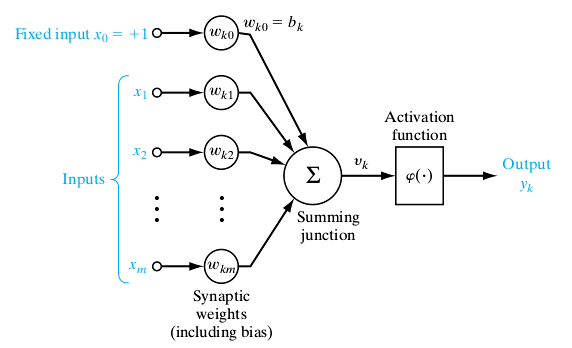
\includegraphics[width=12cm]{imgs/cont_neuron}\\
Ako chybovú funkciu si opäť môžeme zvoliť $1/2 \sum_p (d^{(p)}- y^{(p)})^2$ kde $d^{(p)}$ je $p$-ty očakávaný výstup. Aby naše výsledky boli čo najpresnejšie chceme chybovú funkciu minimalizovať. Na to používame algoritmus gradient descent, ktorý funguje tak, že nájdeme deriváciu chybovej funkcie a v smere proti gradientu budeme meniť váhy tak, aby sme sa dostali na gradient rovný 0. Keď použijeme algoritmus najstrmšieho spádu uvažujú sa dve varianty:
\begin{enumerate}
\item Stochastic gradient descent - po každom videnom príklade spravím update parametrov - $w_j(t+1) = w_j(t) + \alpha(d^{(p)} - y^{(p)})f'x_j = w_j(t) + \alpha\delta x_j$. 
\item Batch gradient descent - prejdeme cez všetky trénovacie príklady spočítame chyby a až potom spravíme update $w_j(t+1) = w_j(t) + \alpha \sum_p \delta x_j$.
\end{enumerate}
Pri stochastickej verzii sice skonvergujeme ale nemusíme sa dostať až do úplného minima ale budeme niekde okolo neho poskakovať. Pri batch verzii robíme najstrmší krok v chybovom priestore a zmenšujeme chybu ako sa len dá, no platíme za to dlším časom počítania. \\\\
Ako dalšie často používané chybové funkcie môžeme spomenúť cross-entropy chybovú funkciu $$-\sum_p [d^{(p)} ln (y^{(p)}) + (1 - d^{(p)})ln(1-y^{(p)})]$$, ktorú keď minimalizujeme dostaneme opäť rovnaké učiace pravidlo ako pri squared error. Táto funkcia nám vlastne povie s akou pravdepodbnosťou príklad patrí do triedy 1 alebo 0.

Tato chybová funkcia je vhodná pri binárnej klasifikácii. Ďaľšou funkciou je softmax $y_i = \frac{exp(net_i)}{\sum_j exp(net_j)}$, ktorá je vhodná napríklad pri klasifikácii do viacerých tried. Potom nám vlastne hovorí s akou pravdepodobnosťou sample patrí do ktorej triedy.
\\\\ \textcolor{red}{TODO} súvis s bayes klasifikatorom.

\subsection{Viacvrstvové dopredné neurónové siete: architektúra a aktivačné vzorce, odvodenie metódy učenia pomocou spätného šírenia chýb (BP) pre dvojvrstvovú doprednú NS, modifikácie BP, typy úloh pre použitie doprednej NS.}
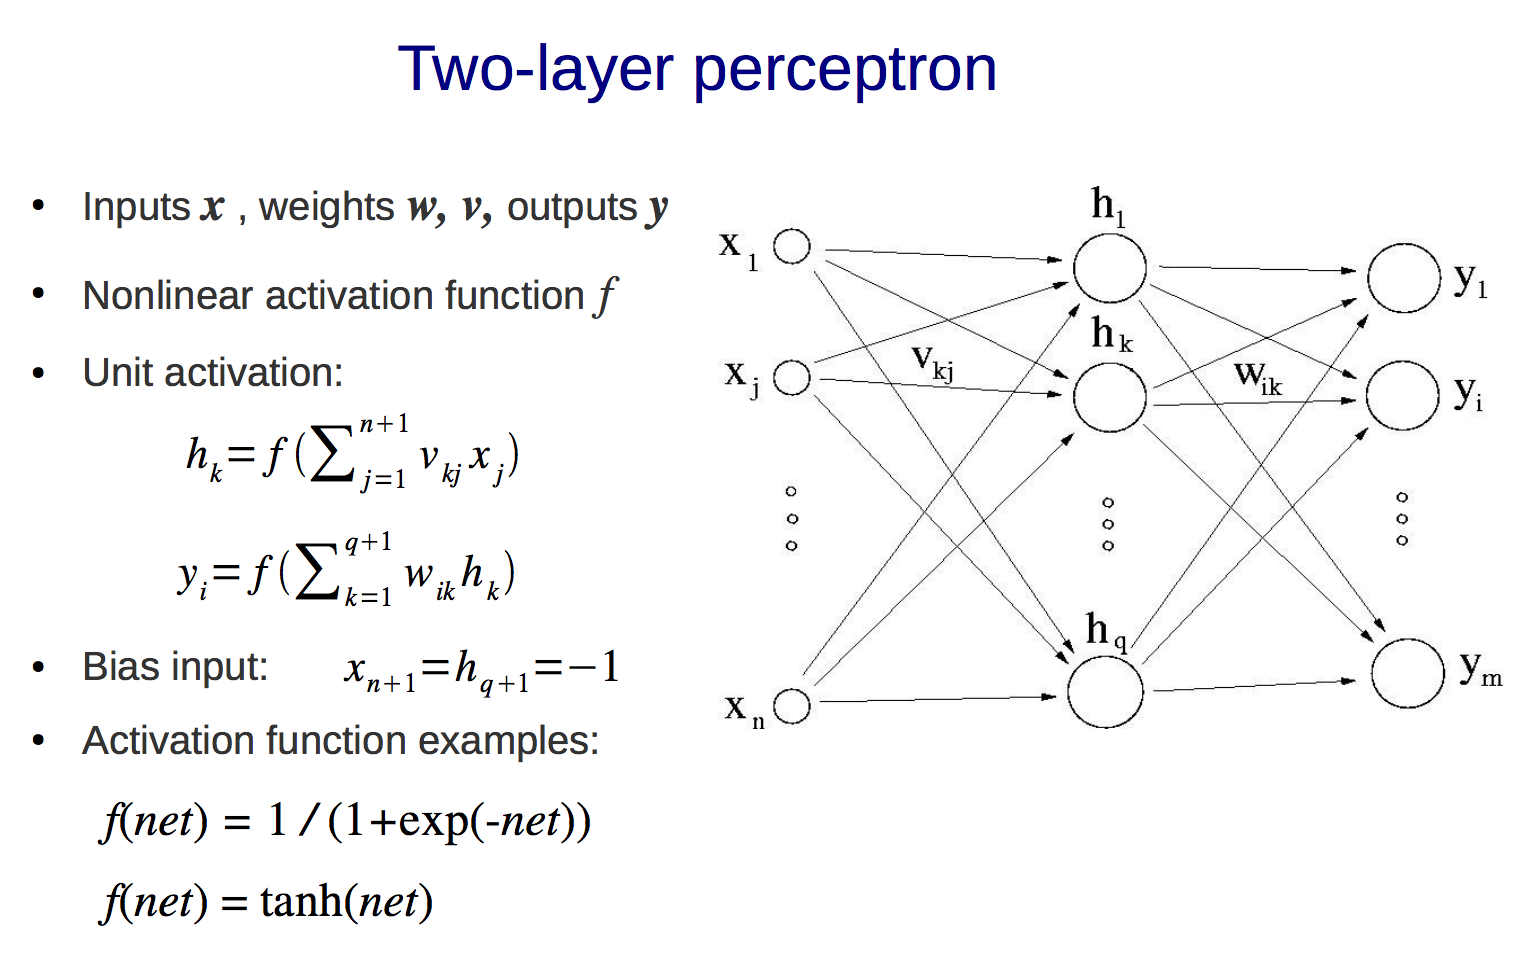
\includegraphics[width=12cm]{imgs/2Lmlp}\\
Otázkou je ako natrénujeme takúto sieť? Ako príklad si zoberme, že chceme minimalizovať kvadratickú chybu $\frac{1}{2}\sum_i(d^{(p)} - y^{(p)})$ na vyššie uvedenom modeli. 
\\\\
Algoritmus error backpropagation(spatné šírenie chyby) používame na natrénovanie dopredných neurónových sietí. Algoritmus vyzerá nasledovne:\\
\begin{enumerate}
\item Vstup - trénovacia množina $\{x^{(p)}, d^{(p)}\}$
\item Inicializácia siete - náhodné váhy a nastavenie rýchlosti učenia, prípadne dalších parametrov
\item Vyber si vstup $x^{(p)}$ a spočítaj výstup $y^{(p)}$. (Forward pass)
\item Vyhodnoť chybovú funkciu $e(t)$.  $E \leftarrow E + e(t)$
\item Spočítaj $\delta_i$ a $\delta_k$ (backward pass)
\item Uprav výhy podla vzťahu ktorý je nižšie.
\item Ak sme použili všetky trénovacie dáta choď na 8. inak na 3.
\item Ak je zastavovacie kritérium splnené	skonči inak spermutuj trénovaciu množinu a začni znova od 1
\end{enumerate}
Učiace pravidlá pre výstupnú a skrytú vrstvu sú rozdielne. Odvodiť by sme ich vedeli napríklad tak, že by sme derivovali chybovú funkciu siete. Backpropagation je v podstate to iste ako metóda najväčšieho spádu.
\begin{itemize}
\item Výstupná vrstva - $ w_{ik}(t+1) = w_{ik}(t) + \alpha\delta_ih_k $, kde $\delta_i = (d_i - y_i)f_i'$.
\item Skrytá vrstva - $ w_{kj}(t+1) = w_{ik}(t) + \alpha\delta_kx_j $, kde $\delta_k = (\sum_iw_{ik}\delta_i)f_i'$.
\end{itemize}
Medzi aplikácie MLP môžeme zaradiť, rozpoznávanie ručne písaných PSČ, spracovanie obrazu(klasifikácia), čítanie anglického textu, etc...

\subsection{Viacvrstvová dopredná NS ako univerzálny aproximátor funkcií (formulácia teorému), trénovacia a testovacia množina, generalizácia, preučenie, skoré zastavenie učenia, selekcia modelu, validácia modelu. Hlboké učenie NS.}
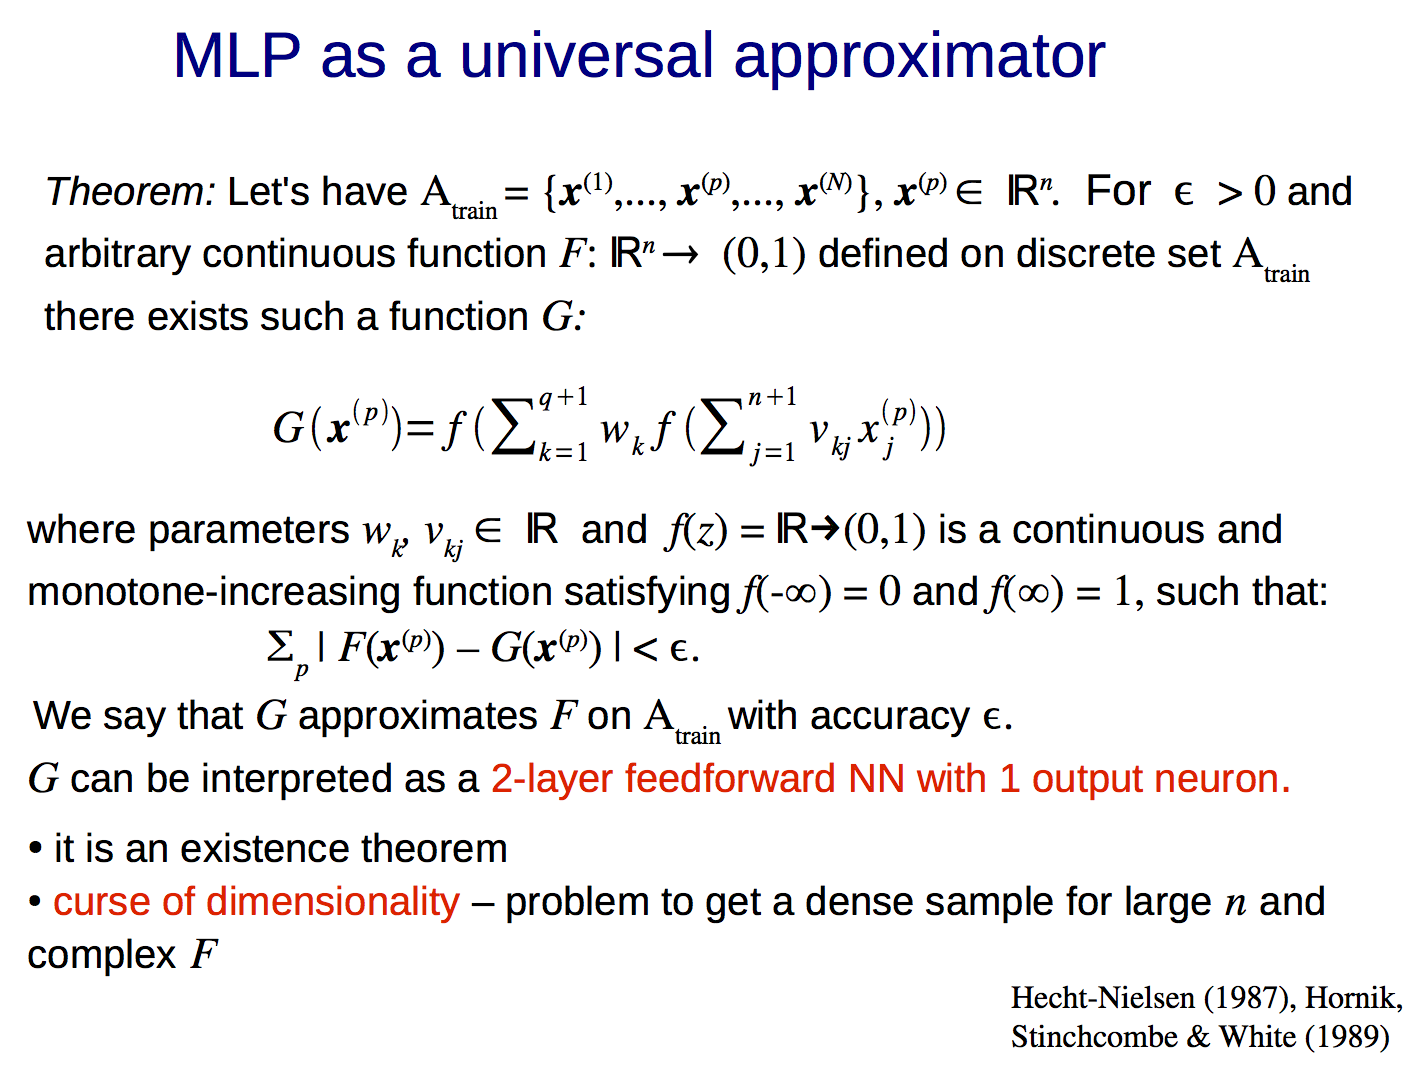
\includegraphics[width=12cm]{imgs/uni_aprox}\\
Trénovacou množinou rozumieme dáta, ktoré používame na trénovanie modelu(minimalizáciu chyby). Zvyčajne pri trénovaní modelu trénovacie dáta náhodne rozdelíme na trénovacie a validačné. Na trénovacích dátach optimalizujeme model a jeho úspešnosť vyhodnocujeme na validačných dátach. Treba si uvedomiť, že validačné a testovacie dáta nie su to isté. Validačné používame na odhad generalizácie modelu a testovacie používame až úplne na konci keď už máme nájdený optimálny model a to tak, že na nich vyhodnotíme jeho úspešnosť.
\\\\
Pod pojmom generalizácia máme na mysli odolnosť modelu voči náhodnému šumu alebo aj výkonnosť modelu na nových dátach. K pojmu generalizácia sa viažu pojmy podučenie a preučnie. K podučeniu dochádza keď náš model nemá dostatočnú silu na aproximovanie náhodného rozdelenia, z ktorého sú dáta samplované. Ako príklad by sme mohli uviesť použitie jednoduchého perceptrónu na problem XOR. Naopak k preučeniu dochádza keď náš model je natolko silný, že sa snaží modelovať náhodný šum v dátach. V ľavo môžeme vidieť dobrý model a vpravo preučený.\\
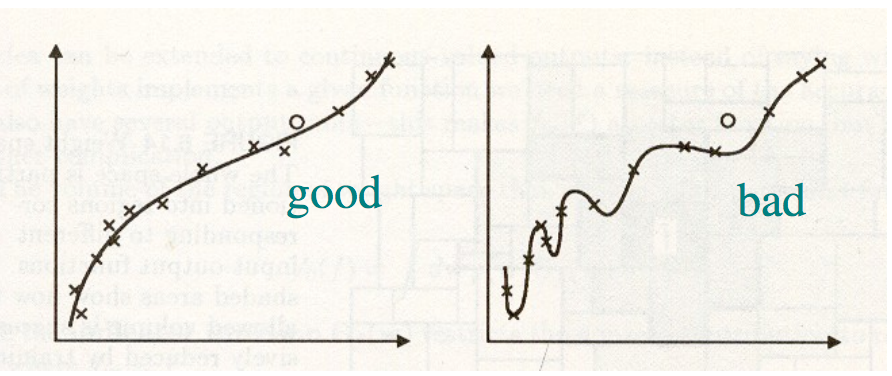
\includegraphics[width=12cm]{imgs/bias_var}\\
Proti preučeniu sa dá bojovať rôznymi spôsobmi, jednak môžeme použiť skoré zastavenie modelu, čo je technika ktorá po každých pár epochách vyhodnocuje validačnú chybu. V prpade, že validačná chyba začne stúpať vrátime sa o krok späť a ukončíme trénovanie.
\\\\
Ďalším spôsobom boja proti preučeniu je takzvaná regularizácia, pri ktorej sa môžeme napríklad snažiť penalizovať velké váhy pri jednotlivých neurónoch(jeden neurón má velký vplyv na výsledok).
\\\\
Pri selekcii modelu potrebujeme zistiť nastavenie rôznych parametrov ako je počet vrstiev a počet neurónov v nich, rýchlosť učenia poprípade iné parametre. Vhodnou metódou zisťovania úspešnosti modelu je k-fold cross validation, čo je metóda pri ktorej rozdelíme dáta na náhodných $k$ podmnožín. Následne vyberem $k-1$ z nich na ktorých model natrénujem a poslednú podmnožinu použijem na validáciu úspešnosti modelu. Toto spravím $k$ krát - zakaždým trénujem a validujem na inej podmnožine. Suma sumárum dostanem $k$ rôznych validačných hodnôt. Tie sa zvyknú spriemerovať a poprípade sa z nich zvykne vypočítať ešte aj smerodajná odchýlka. 
\\
Tento postup zopakujem pre všetky možnosti uvažovaných parametrov a vyberem model, ktorý ma najmenšiu priemernú chybu, prípadne vezmem do úvahy aj smerodajnú odchylku.
\\\\
Pod pojmom deep learning sa rozumejú siete, ktoré majú viac vrstiev.

\subsection{Lineárne modely NS: vzťah pre riešenie systému lin. rovníc v jednovrstvovej sieti, pojem pseudoinverzie matice, autoasociatívna pamäť: lineárny obal, princíp funkcie modelu, detektor novosti.}
Nech máme trénovaciu množinu $A_{train} = \{ (x^{(p)}, y^{(p)}), p=1,\cdots,N \}$ a hľadáme maticu $W$, ktorá spĺňa $$y^{(p)} = Wx^{(p)}, \forall p$$

V maticovej notácii $$Y = WX$$ potom riešenie systému vieme jednoducho nájsť tým, že prenásobíme takýto systém inverznou maticou k matici $X$ zprava a dostaneme teda $$YX^{-1} = W.$$Probém je v hľadaní inverznej matice k matici X pretože táto matica nemusí byť regulárna. Z tohto dôvodu sa zaviedol pojem pseudoinverznej(Moore-Penrose) matice, ktorú označujeme $X^+$. A má nasledovné vlastnosti ($\forall X \exists X^+$ )
\begin{enumerate}
\item $XX^+X = X$
\item $X^+XX^+ = X^+$
\item $X^+X$ a $XX^+$ sú symetrické
\end{enumerate}
Vypočítat ich potom môžeme nasledovne
\begin{enumerate}
\item $X^+ = X^T(XX^T)^{-1}$ ak n < N a hodnost(X) = n.
\item $X^+ = (X^TX)^{-1}X^T$ ak n > N a hodnost(X) = N.
\end{enumerate}
kde $N$ je počet príkladov a $n$ je dimenzia vstupu.
\\\\
Chceli by sme natrénovať model X = WX, $N < n$ a chceme aby model vedel rekonštruovať N vstupov. Takýto model voláme lineárny autoasociátor. V prípade, že $N=n$ by sme dostali triviálne  riešenie $W = I$, to ale nie je to čo chceme. Keď dostaneme zašumený vstup tak chceme odpovedať zapamätaným vzorom. 
\\\\
Linear manifold $L = \{ x \in R^n | x = a_1x_1 + a_2x_2 + \cdots + a_Nx_N, a_p \neq 0 \} , L \subset R^n$ \\
Ortogonálny komplement = $L^{\perp} = \{x \in R^n | x \perp L\}$ \\
A taktiež platí, že : $L \cup L^\perp = R^n$
\\\\
Každý vektor z $X$ vieme jednoznačne rozložiť na $ x = x_{obal} + x_{orto}$ kde $x_{obal} \in L, x_{orto} \in L^{\perp}$.Tréningová množina $X = \{ x_1, x_2, \cdots, x_n\}$ bude tvoriť náš lineárny obal $L$. Teraz keď dostaneme ľubovoľný vstup $x$, predpokladajme, že je zašumený, ale keďže ho vieme rozložiť tak nám stačí spraviť ortogonálnu projekciu $Wx = (XX^+)x = x_p$, čím dostaneme pattern ktorý je najbližšie danému vektoru. V prípade, že by sme spočítali $Wx = (I - XX^+)x = x_p$ potom $x_p \in L^{\perp}$, toto voláme detektor novosti.


\subsection{Lineárne modely NS: účel Grammovho-Schmidtovho ortogonalizačného procesu, GI model. Pamäť korelačnej matice ako autoasociatívna pamäť, vzťah pre výpočet váh, presluch, porovnanie s GI.}

\textbf{Gramm-Schidtov ortogonalizačný proces} vytvorí z báze $u_1, u_2, \dots u_n$ ortogonálnu bázu $v_1, v_2, \dots v_n$ takto:
$$v_1 = u_1$$
$$v_2 = u_2 - \frac{v_1^Tu_2}{|v_1|^2}$$
$$v_k = u_k - \sum_{i=1}^{k-1}{\frac{v_i^Tu_k}{|v_i|^2}}$$

\textbf{General Inverse model}: 
Na to aby sme pridali ďalší vektor do lineárneho obal nepotrebujeme ho vždy nanovo prepočítať, ale stačí pridať nový vektor pomocou nasledujúceho postupu:


Nech $\widetilde{x}_1, \widetilde{x}_2 \dots \widetilde{x}_n$ sú vektory určené zo vstupov $x_1, x_2 \dots x_n$:
$$W(0) = 0$$

$$W(n+1) = W(n) + \frac{\widetilde{x}_{n+1} \widetilde{x}_{n+1}^T}{|\widetilde{x}_{n+1}|^2}$$

Kde $\widetilde{x}_{n+1} = x_{n+1} - W_n x_{n+1}$
\\\\
\textbf{Pamäť korelačnej matice}\\
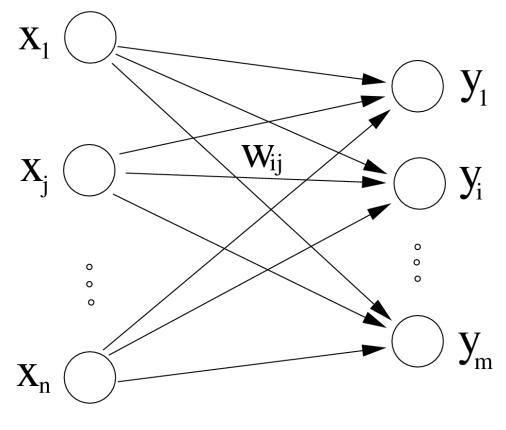
\includegraphics[width=8cm]{imgs/cmm}\\
Váha $w_{ij}$ je priamo  umerna korelacii: $w_{ij} \approx \sum_{k=1}^n x_{j}^ky_{i}^k$ čo sa v maticovom prevedení dá napísať ako $W \approx YX^T$. Uvažujme, ale autoasociatívny prípad: $W \approx X X^T$ a ak sú vstupné vektory ortonormálne dostávame $X^T = X^{-1} = X^+$ a tento model je totožný s GI.

Rekurzívny výpočet CMM (Correlation matrix memory):
$$W(n+1) = W(n) + x^{(n+1)}  x^{(n+1)T}$$

\textbf{Presluch} sa dá vyjadruje takto: 

Odpoveď na vstup ľubovoľné vstup $x_p$ je vyjadrená: $$Wx^p = X X^T x^p = \sum_{k=1}^n x^k x^{kT} x^p = x^p x^{pT} x^p + \sum{k=1;k!=p}^n x^k x^{kT} x^p = x^p |x^p|^2 + C(p)$$ a práve C(p) označuje presluch. Ak by bol presluch nulový tak vstupy $x_1 \dots x_2$ sú ortogonálne. Hodnota presluchu sa dá znížiť posunutím strednej hodnoty zložiek vstupov do nuly.

Krátke vysvetlenie: CMM sa snaží zachytiť korelácie medzi jednotlivými zložkami a na základe nich previazať vstupy zo vstupnej na výstupnú vrstvu (vyššia korelácia => vyššia hodnota váhy). Model sa opiera iba o previazanosti medzi dvojicami a nie previazanosti napr. trojíc, štvoríc, .... 
\textbf{Porovnanie}
Ak sú vsupy dostatočne odlišné tak CMM je rýchlejšia alternatíva ku GI. Ale inak GI dáva lepšie výsledky. 

\section{Samoorganizácia a RBF sieť. Otázky 8 až 12.}
\subsection{Samoorganizácia v NS, základné princípy, pojem učenia bez učiteľa, typy úloh použitia, Ojovo pravidlo učenia pre jeden neurón, vysvetlenie konvergencie.}

4 základne princípy samoorganizácie:
\begin{enumerate}
\item Samo-zosilnenie,  zmena váh ma sklon k zosilneniu
\item Konkurencia - medzi neurónmi, vzhľadom na obmedzené zdroje
\item Spolupráca – medzi susednými neurónmi
\item Konštrukčná informácia – je získavaná zo vstupných dát ako „knowledge“
\end{enumerate}
Učenie bez učiteľa je algoritmus učenia, ktorý nemá informáciu o požadovaných aktivitách výstupných neurónov v priebehu trénovania o ktoré by sa mohol opierať. Pojem učenie bez učiteľa sa používa na opis širokej škály rôznych učiacich sa úloh. Úlohy tohto typu analyzujú sadu objektov, ktoré nemajú priradenú triedu.
\\\\
Typy úloh:
\begin{itemize}
\item Klasterizácia údajov (vektorová kvantizácia)
\item PCA, redukcia dimenzie pričom sa snažíme čo najviac zachovať vzájomné vzťahy
\item Topologické zobrazenie príznakov
\item Kompresia dát, tak aby sme zachovali čo najviac z pôvodných
\end{itemize}
Predpokladajme, že máme jeden neurón s $n$ vstpmi $y = \sum_{j=1}^n w_jx_j = \textbf{w}^T\textbf{x}$
Ojovo pravidlo je pravidlo, ktoré hovorí o zmene váh medzi neurónmi. Je to modifikácia štandardného Hebbovho pravidla a vyzerá nasledovne:
$$w_j(t+1) = \frac{w_j(t) + \alpha yx_j}{||\textbf{w(t)} + \alpha y\textbf{x}||}$$
Pre malé $\alpha$ môžeme pomocou taylorovho rozvoja zapísať aj v tvare:
$$w_j(t+1)= w_j(t)+\alpha yx_j - y^2w_j(t)$$
\\\\
V prípade jedného neurónu, jeho váhový vektor $w$ konverguje k vlastnému vektoru matice $R<xx^T>$ alebo k prvému hlavnému komponentu. Rozptyl nášho neurónu $\sigma2(n) = <y^2(n)>$, potom konverguje k hlavnému vlastnému číslu.
\textcolor{red}{TODO konvergencia nedostatočná}

\subsection{Metóda hlavných komponentov pomocou algoritmu GHA a APEX, architektúra modelu, vzťah pre adaptáciu váh, pojem vlastných vektorov a vlastných čísel, redukcia dimenzie, aplikácia na kompresiu obrazu.}

Metóda hlavných komponentov nám v priestore parametrov trénovacích dát nájde také smery, v ktorých majú dáta najväčšiu varianciu. Následne keď chceme redukovať dimenzionalitu pristoru predpokladáme, že smery s najvačšou varianciou sú najdôležitejšie.
\\\\
Pozrime sa na algoritmus GHA. Architektúra modelu GHA je jednovrstvová sieť s $n$ vstupmi a $p$ výstupmi. Generalizovaný Hebbovský algoritmus na aktualizáciu váh je v tvare
 $$\Delta w_{ij} = \alpha y_i(x_j - \sum_{k=1}^p y_kw_{kj}).$$
To čo GHA robí je, že extraktuje $p$ hlavných komponentov korelačnej matice vstupných dát. Výhodou oproti klasickému PCA je, že nemusíme počítať korelačnú maticu a zároveň je to výpočtovo o dosť lacnejšie ak máme prípad $p << n$. Taktiež sa dá dokázať, že po skonvergovaní dostaneme usporiadané hlavné komponenty a taktiež, že výsledok je reprodukovatelný až na znamienka. 
\\\\
Adaptive Principal component EXtraction(APEX) - je algoritmus, ktorý používa opačný spôsob učenia, tj. anti-Hebbovské učenie. Architektúra siete je opať jednovrstvová ale teraz má naviac laterálne spojenia(v rovnakej vrstve). Hlavné komponenty hľadá iteratívnym prípstupom, že keď by dostala $i-1$ hlavných komponentov tak z nich vypočíta $i$-ty hlavný komponent. $I$-ty neurón má teda okrem klasických váh $w_i$ aj laterálne $$u_i = [u_{i1}, \dots, u_{i-1}]^T.$$ Výstup siete spočítame pomocou vzťahu 
$$ \textbf{y}_i = \textbf{w}_i^T\textbf{x} + \textbf{u}_i^T\textbf{y}_{i-1}, \text{  kde } \textbf{y}_{i-1} = [y_1, y_2, \dots, y_{i-1}]^T. $$
Aby sme našli hlavné komponenty, dopredné váhy trénujeme pomocou Ojovho pravidla a laterálne váhy pomocou anti-Hebbovského pravidla(inhibičného), ktoré má tvar podobne ako klasické Hebbovské pravidlo akurát je tam mínus: $$ \Delta u_{ik}= -\alpha y_i(y_k + y_iu_{ik}). $$
Keď to správne naimplementujeme, dopredné váhy by mali konvergovať k vlastným vektorom korelačnej matice vstupov a laterálne interakcie k nulovému vektoru.
\\\\
Nech máme ľubovoľný obrázok vieme ho previesť do šedotónového. Následne môžeme na podobrázkoch velkosti 8x8 spustiť naše PCA algoritmy, ktoré nájdu vlastné vektory k týmto podobrázkom. To čo vidím, že sa deje je nejaká forma rasterizácie.

\subsection{Učenie so súťažením (typu “winner-take-all”), nevýhody. Neurobiologická motivácia algoritmu SOM, laterálna interakcia a jej náhrada v SOM, sumarizácia algoritmu, voľba parametrov modelu.}
Učenie so súťažením je biologicky motivované tak, že čím viac sa synapsie používajú tým by mali byť silnejšie. Výskumníci sa tiež inšpirovali modelom toho ako sietnica mapuje svoje impulzy v mozgu. Model samoorganizujúcej sa mapy(SOM) je model s dvomi vrstvami, vstupnou a výstupnou. Výstupná vrstva zvykne byť vačšinou organizovaná v mriežke, najčastejšie 2D(kvôli vizualizácii) ale občas sa využíva aj viac D mriežka. Každý neurón na vstupnej vrstve je prepojený s každým na výstupnej. \\
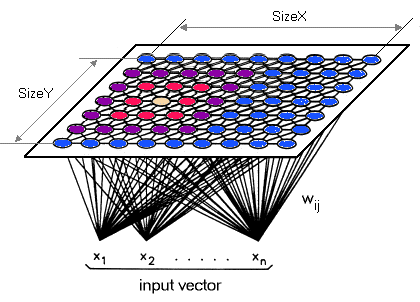
\includegraphics[width=12cm]{imgs/som}\\
V prípade učenia typu “winner-take-all” sa ku každému vstupnému vzoru nájde jeden neuón(tzn. BMU - best matching unit) $bmu_c = max_i\{\textbf{w}_i^T\textbf{x}\}$, ktorý je následne pritiahnutý vstupným vzorom k sebe $\Delta w_c = \alpha (x - w_c)$. Nevýhodou tohto prístupu je, že veľa neurónov ostane na svojej pôvodnej pozícii a v podstate ničomu nepomáhajú(dead neurons).\\\\
Neskôr sa vymyslelo, že neuróny budú mať v mriežke topológiu(umiestnenie) a budeme sa učiť spôsobom "winner-take-most" tak, že neuróny v okolí budú spolupracovať. V prípade, že sú blízko vzruchu a spojenie sa využíva tak ho posilňujeme v opačnom prípade ho potlačujeme. Túto spoluprácu nazývame laterálna interakcia. V SOM-ke sme to nahradili výpočtovo efektívnejším modelom tak, že upravujeme iba neuróny v určitom okolí BMU, a okolie sa s postupným časom učenia zmenšuje. Ako príklad funkcie okolia si môžeme uviesť napríklad "rectangular neighbourhood"\\
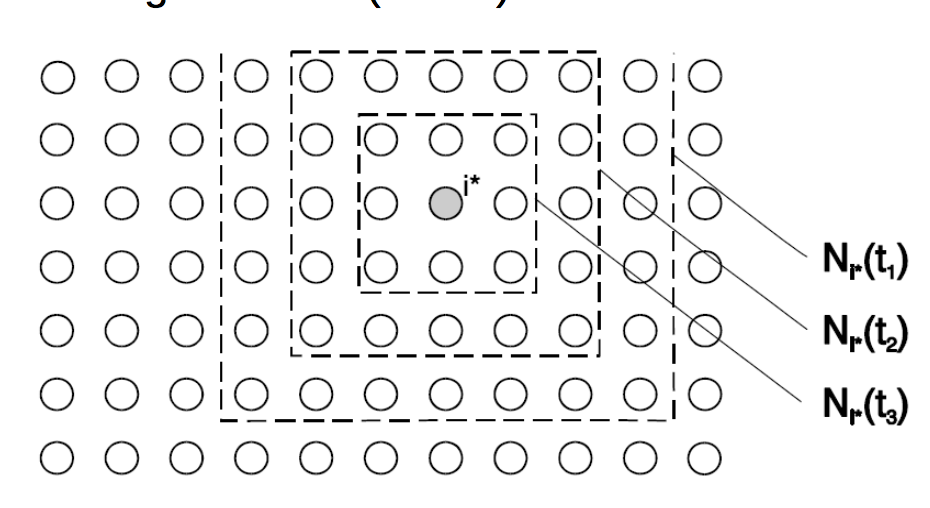
\includegraphics[width=12cm]{imgs/rect_neighb}\\
Alebo alternatívne gausovské okolie dané vzťahom $h(i^*, i) = exp(\frac{d^2_E(i^*, i)}{\lambda^2}(t))$, kde lambda sa postupne zmenšuje $\lambda(t) = \lambda_i(\frac{\lambda_f}{\lambda_i})^{t/t_{max}}$. \\
$\lambda_i$ je lambda na začiatku výpočtu a $\lambda_f$ je lambda na konci výpočtu. $t$ a $t_{max}$ je aktuálna iterácia a celkový počet iterácii.
\\\\
Suma sumárum algoritmus vyzerá nasledovne:
\begin{itemize}
\item Zoberieme náhodný vstup $x$ a najdeme k nemu BMU $$i^* = arg min_i ||x - w_i||.$$
\item Upravíme na základe BMU váhy : $$ w_i(t+1) = w_i(t) + \alpha(t)h(i^*,i)[x(t) - w_i(t)] $$
\item Updatneme parametre(susednost, rychlost ucenia) SOM a opakujeme do konvergencie.
\end{itemize}
\subsection{SOM: vektorová kvantizácia, topografické zobrazenie príznakov, algoritmus SOM, parametre, redukcia dimenzie, magnifikačná vlastnosť, príklad použitia.}
Úlohou vektorovej kvantizácie je nahradiť množinu vstupných dát X množinou referenčných vektorov takzvaných prototypov. To znamená že namiesto pamätania si celej množiny vstupných dát stačí si pamätať oveľa menšiu množinu prototypov. Zároveň si treba aj pamätať príslušnosť každého vstupného vektoru k jednému z prototypov (k tomu ku ktorému je najbližšie, Euklidovská vzdialenosť). Touto kvantizáciou nám vznikne tzv. Voronoiho mozaika.
\\\\
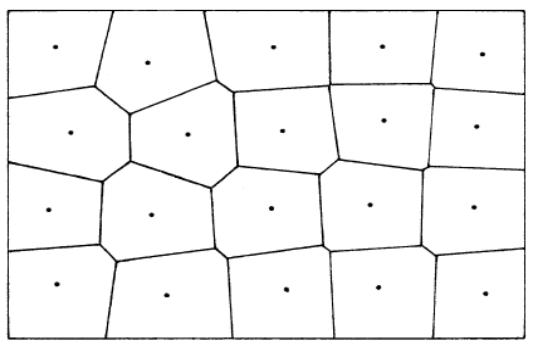
\includegraphics[width=12cm]{imgs/voronoi}\\
Bodky sú prototypy a ku každému prototypu prislúcha oblasť vstupných dát ktoré prislúchajú danému prototypu.
Kritériom vektorovej kvantizácie je nájdenie optimálnych pozícií týchto prototypov. Ak sa pozeráme na prototypy ako na váhové vektory, predstavuje algoritmus SOM štandardný vektorový kvantifikátor.
\\\\
Oba algoritmy PCA aj SOM umožňujú extrahovať hlavné príznaky, hlavné črty vstupných dát. Účelom extrakcie hlavých príznakov je predovšetkým redukcia dimenzie pričom sa snažíme čo najviac zachovať vzájomné vzťahy. Redukciou dimenzie sa uľahčí spracovávanie dát a zároveň získame možnosť vizualizácie.
Okrem iného, rozdiel medzi PCA a SOM spočíva v spôsobe reprezentácie príznakov. Pri
PCA je na reprezentáciu jedného príznaku použitý len jeden neurón (hodnota príznakov je
kvantifikovaná výstupmi neurónov), v prípade SOM sa na reprezentácii podieľajú všetky
neuróny (hodnota príznakov je daná pozíciou víťaza). S tým súvisí špecifická vlastnosť
SOM - extrahované príznaky sú topologicky zobrazované (angl. feature mapping), a to
pozdĺž koordinát mriežky SOM.
\\\\
Magnifikačná vlastnosť je vlastnosť mapy aproximovať čo najlepšie distribúciu vstupných dát. V oblastiach kde sú zhustené vstupné dáta bude tak isto zhustené rozloženie váhových vektorov siete. Takúto tendenciu algoritmu SOM možno interpretovať ako snahu o optimálne rozloženie svojich zdrojov. Túto vlastnosť algoritmu popisuje magnifikačný faktor, počet  váhových vektorov pripadajúcich na jednotkovú plochu vstupného priestoru.\\
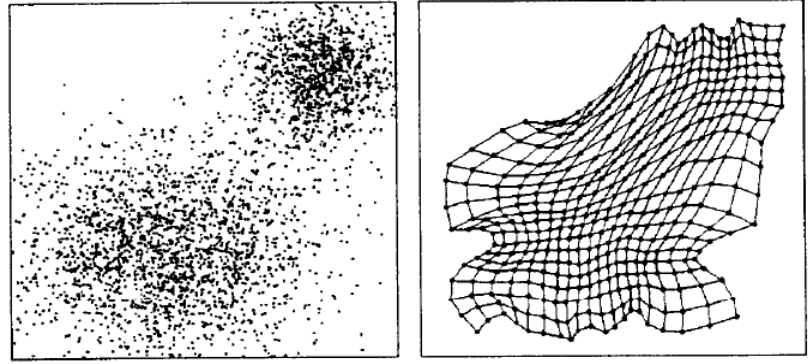
\includegraphics[width=12cm]{imgs/magnif}
\\\\
Aplikácií SOM je veľa. Spomenuli sme rozpoznávanie reči a robotiku. Pri rozpoznávaní reči sme transformovali akustický rečový signál na sekvenciu hlások pričom sme si vytvorili tzv. fonémovú mapu. Pri robotickom ramene je úlohou dostať koncový bod ramena do určitej pozície. Obrázky sú na slajdoch ale nemyslím si že to chce podrobne vysvetliť.

\subsection{Hybridné modely NS, RBF model: aktivačné vzorce, bázové funkcie, príznakový priestor, problém interpolácie, trénovanie modelu, aproximačné vlastnosti RBF siete.}
Tento model je istou kombináciou učenia s učiteľom a bez učiteľa. Funguje to veľmi dobre pokiaľ pre podobné vstupy očakávame podobné výstupy. Väčšinou vyžadujeme viac neurónov ako pri ostatných modeloch učených iba s učiteľom. Konkrétne sa pozrieme na model Radial Basis Function neural network.
\\\\
Tradične máme vstupy $x$, váhy $w$ a výstupy $y$.\\
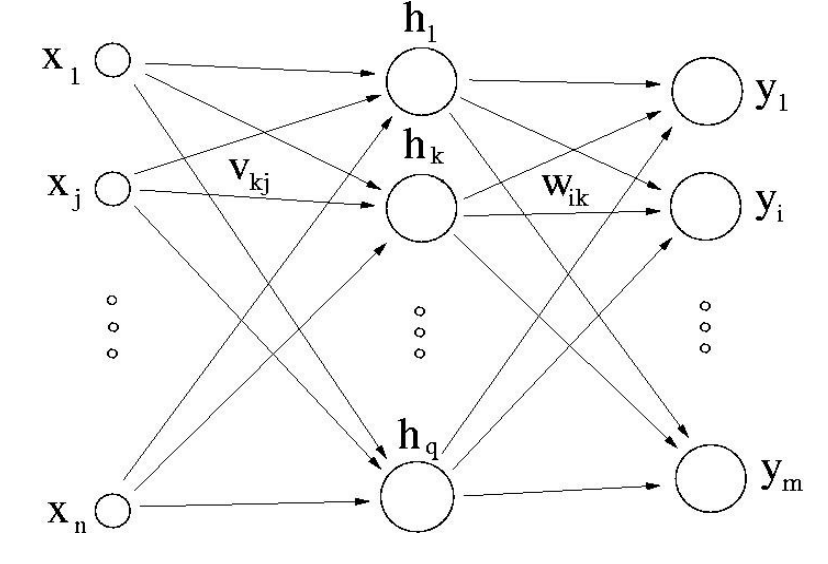
\includegraphics[width=10cm]{imgs/rbf}\\
Výstupné aktivácie budú teda podla schémy
 $$y_i = \sum^q_{k=1}w_{ik}h_k(x) + w_{i0} $$, kde $h_k$ je radiálna aktivačná funkcia, ako napríklad $exp(-\frac{||x-v_k||^2}{\sigma_k^2})$, $v_k$ je centrum $k$ a $\sigma_k$ je rozsah. 
\\\\
Cover theorem: \\
A complex pattern classification problem cast in a high dimension space nonlinearly is more likely to be lineary separable than in low dim. space.
\\\\
Interpolation problem:\\
Pre RBF v podstate dostaneme systém lineárnych rovníc $\textbf{w}^T\textbf{h}_i = d_i, i=1,2,\dots,N$. Ak $H^{-1}$ existuje potom riešením je $w = H^{-1}d$. Ako si môžeme byť ale istí, že interpolačná matic $H$ nie je singulárna?. Na pomoc nám prichádza Michelliho veta: \\

Nech $x_i \in R^N$ je množina rôznych bodov, potom $H(N\times N)$ ktorej $h_{ij} = \phi_{ij}(||x_i - x_j||)$, nie je singulárna. 

Veľa BRF funkcií túto podmienku spĺňa.
\\\\
Ako príklady bázových funkcií si môžeme uviesť napríklad nasledovné:\\
\begin{itemize}
\item Gaussian $\phi(r) = exp(-\frac{r^2}{\sigma^2})$
\item Multiquadrics $\phi(r) = (r^2 + c^2)^{1/2}$
\item Inverse multiquadrics $\phi(r) =  (r^2 + c^2)^{-1/2}$
\item Cauchey $\phi(r) = \frac{1}{1+r^2}$
\end{itemize}
Park a Sandberg dokázali, že za určitých predpokladov (viz Farkaš slidy 136.) existuje pre každú spojitú funkciu f(x) RBF sieť s centrami $v_k$ a rovnakou veľkosťou $\sigma > 0$ taká, že F(x) je blízko f(x). Tj. taká, ktorá dobre aproximuje funkciu f(x).
\\\\
Trénovanie tejto siete prebieha tak, že rôzne trénujeme prvú vrstvu a inak druhú.
\begin{itemize}
\item 1. vrstva - môžeme trénovať napríklad pomocou K-means alebo inej clustrovacej metódy \\\\
Ak sú dáta distribuované v nejakej štruktúre môžeme použiť napríklad nasledovný vzťah:
$$ G(||x-v_i||^2) = exp(\frac{-K||x-v_i||^2}{d^2_{max}}), $$ kde $K$ je počet centier, $d_{max} = max_{kl}\{||v_k - v_l||\}$\\ 
Alebo môžeme použiť K-means kde centrá položíme randomne alebo na nejaké trénovacie body, pre každý trénovací sample nájdeme víťazný stred a tie zaradíme do jedneho clusteru. Teraz updatneme pozíciu stredov tak aby boli v strede svojho clusteru a opakujeme od zaciatku az do konvergencie.
\item 2. vrstva - pomocou SGD alebo výpočtom pseudoinverznej matice $H'$, kde potom $W = H'D$
\end{itemize}



\section{Rekurentné a pamäťové modely. Otázky 13 až 18.}	
\subsection{NS na spracovanie sekvenčných dát: reprezentácia času, typy úloh pre rekurentné NS. Modely s časovým oknom do minulosti, výhody a nedostatky, príklad použitia.}

Pri spracovaní sekvenčných dát je dôležité, aby výstup siete nebol závislý iba od súčasnej hodnoty, ale aj od predchádzajúcich (prípadne nasledujúcich - bidirectional RNN) hodnôt sekvencie. Tento typ siete je teda vhodný pre riešenie typov úloh, kde výsledok závisí od celého kontextu spracovávaného vstupu. Ide teda napríklad o klasifikácia sekvencií (spracovanie reči - NLP), predikcia alebo generovanie nových sekvencií.
\\\\
\subsubsection{Nerekurentné modely}
Existujú 2 typy sietí - rekurentné (viď ďalšiu otázku) a nerekurentné. Pri nerekurentných modeloch väčšinou hovoríme o dopredných sieťach (MLP), ktoré sa môžu trénovať klasickým back-propagation algoritmom. Aj dopredné siete môžu byť použité na spracovanie sekvencií - použitím tzv. časového okna. Pri tejto technike neplníme sieť iba aktuálnou hodnotou, ale máme fixný počet vstupných neurónov pre predchádzajúce príp. nasledujúce hodnoty sekvencie.
\begin{center}
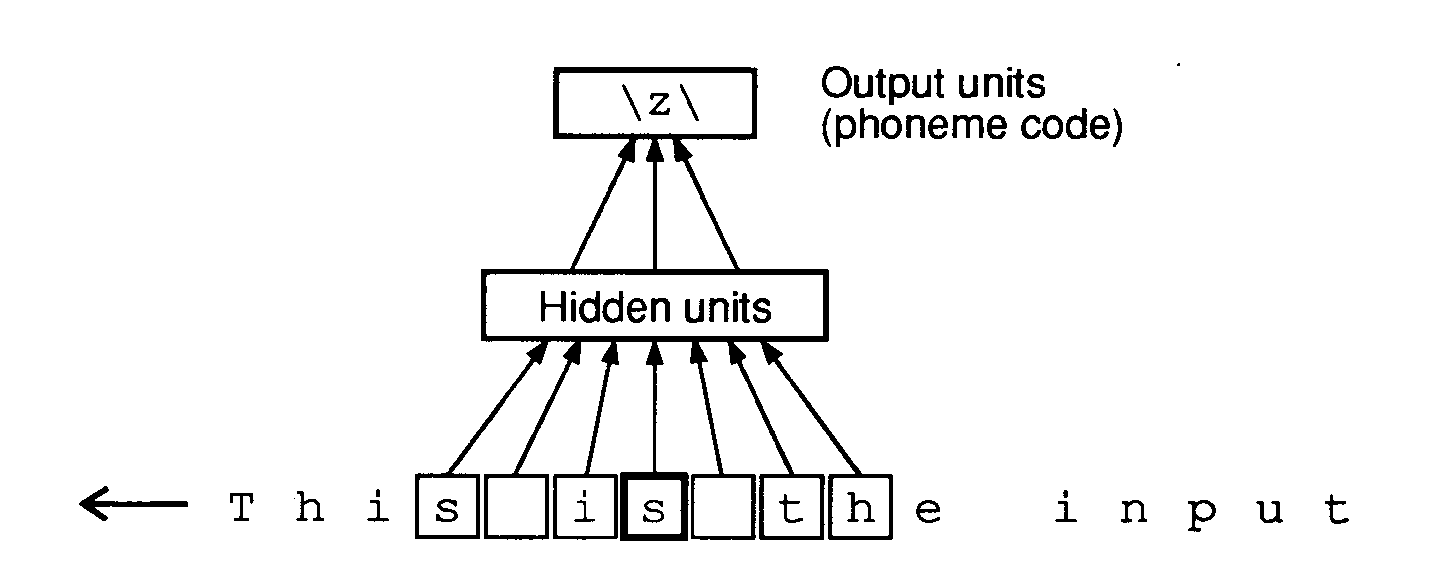
\includegraphics[width=7cm]{imgs/tap}\\
\end{center}
\begin{center}
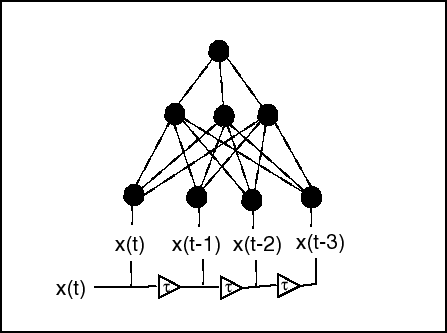
\includegraphics[width=7cm]{imgs/tapped}\\
\end{center}
Tento prístup bol napríklad použitý pri určení výslovnosti anglických hlások (NETtalk), trénovaní FIR filtra (focused neuronal filter alebo rozpoznávanie vyslovených hlások zo spektogramu. Problém pri tomto modely je v tom, že nevie spracovať ľubovolne dlhú sekvenciu - počet vstupných neurónov musí byť fixný a sieť nemá spätnú väzbu od vstupov. Avšak na rozdiel od rekurentných sietí sa jednoduchšie trénuje a nepodlieha napr. problému miznúceho gradientu. 

\subsection{Rekurentné NS: princíp trénovania pomocou algoritmu BPTT a RTRL. Príklad použitia.}
Graf dopredných sietí tvorí DAG, avšak rekurentné siete môžu obsahovať aj cykly. Hlavnou myšlienkou rekurentných sietí je spätná väzba vstupu - určenie stavu v závislosti od predchádzajúcich vstupov. Pomocou nich sa dá napríklad modelovať mealy-ho automat. Je to niečo ako konečný automat z foje - začíname v určitom stave a do dalších stavov sa presúvame v závislosti od aktuálneho vstupu a stavu, v ktorom sa aktuálne nachádzame. Pravidlá týchto prechodov je možné natrénovať vhodnou rekurentnou sieťou (dopredným modelom s časovým oknom do minulosti to zrejme nie je možné).
\begin{center}
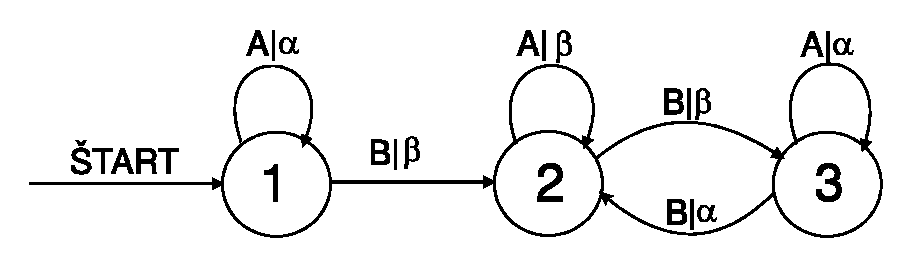
\includegraphics[width=7cm]{imgs/mealy}\\
\end{center}
Medzi čiastočne rekurentné siete s kontextovou jednotkou patrí:
\begin{itemize}
\item Elman - Spätná väzba zo skrytej vrstvy, vie rozpoznať a generovať sekvencie a robiť predikcie. Znázornená na obrázku nižšie. 
\item Jordan - Spätná väzba  výstupnej vrstvy
\item Stornetta - moveing average (MA) predchádzajúcichaktivácií (IIR filter)
\item Mozer - nedá sa použiť Backpropagation


\subsubsection{Back-propagation through time - BPTT}
Rozšírenie klasického BP - rekurentnú sieť "rozbalíme" na doprednú sieť, s hĺbkou rovnou dĺžke sekvencie. 
\begin{center}
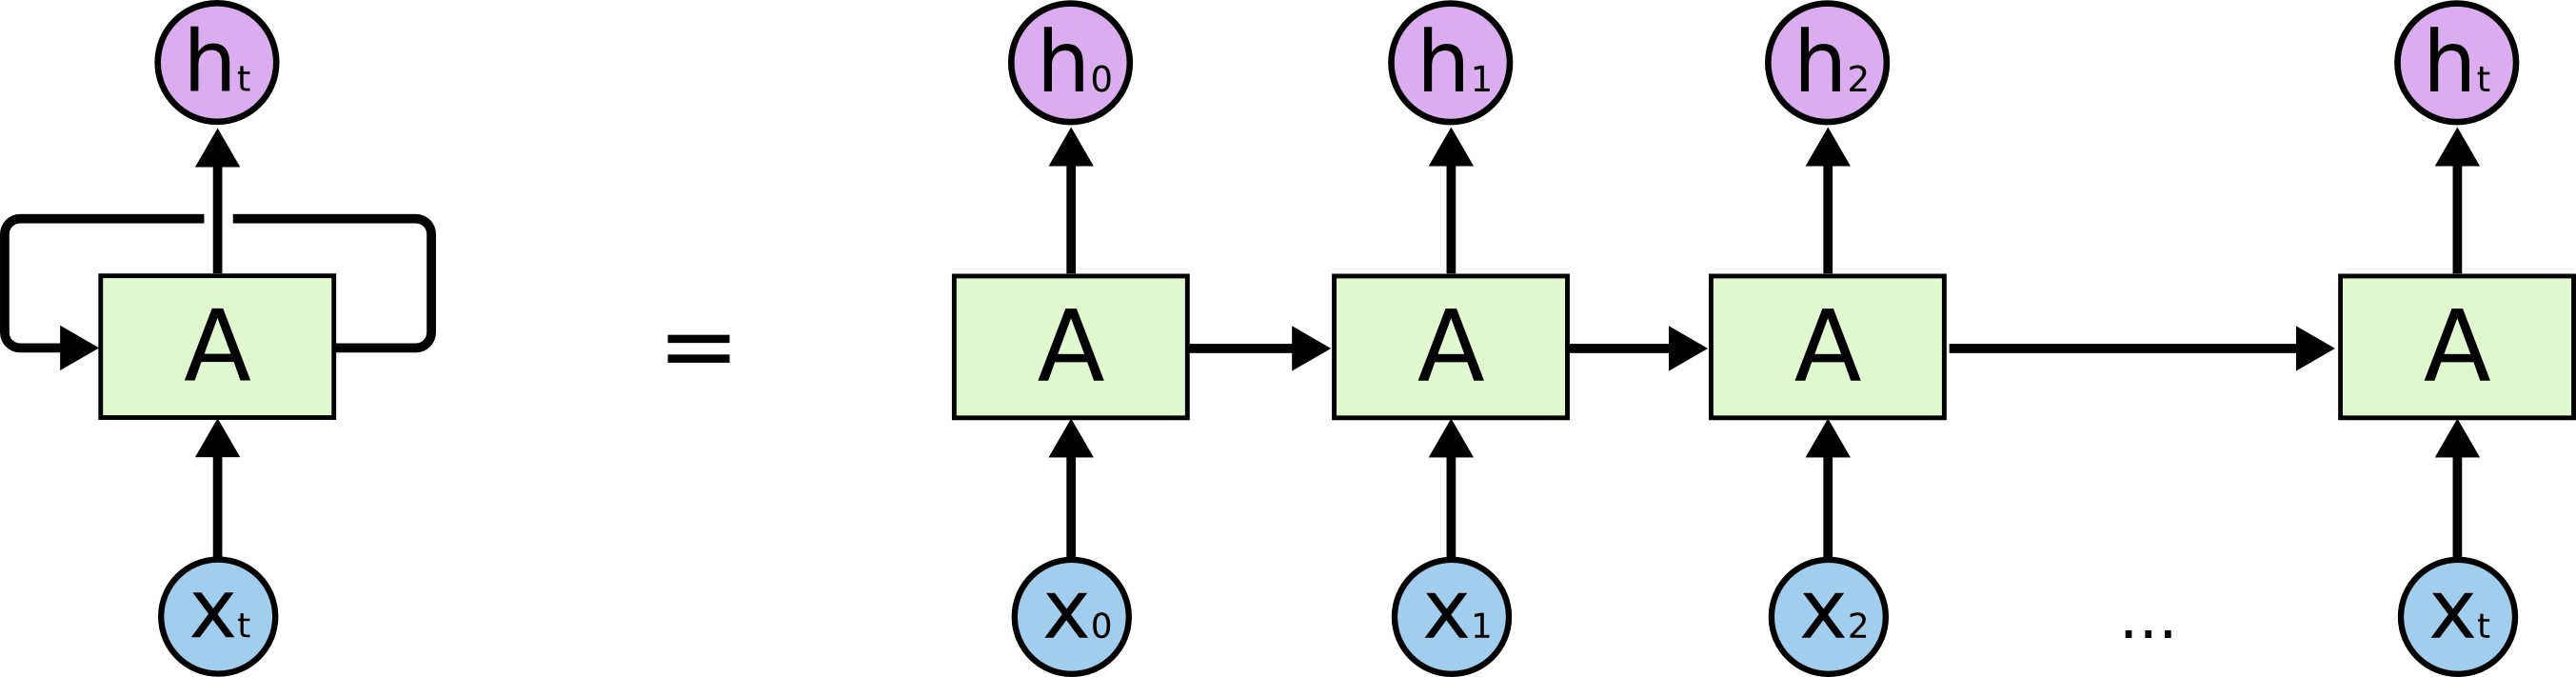
\includegraphics[width=7cm]{imgs/RNN-unrolled}\\
\end{center}
kde $x_i$ reprezentuje vstup, $A$ reprezentuje stav a $h_i$ výstup. Hodnoty stavov sú dané vzťahom:
$$A_i(t+1) = f(\sum_j w_{ij} A_j(t) + x_i(t))$$
Back propagation musí byť aplikovaný po spracovaní každej sekvencie. Cieľom je optimalizovať chybovú funkciu:
$$E(T) = \frac{1}{2} \sum_{t=1}^T \sum_{i \in O} e_i^2(t)$$
kde $T$ je dĺžka sekvencie. Nech:
\begin{numcases}{\delta_i(t) = }
  f'(\textit{net}_i)e_i(t), & $t = T$ \\
  f'(\textit{net}_i)(e_i(t) + \sum_{l \in O} w_{li} \delta_l(t + 1))), & $1 < t < T$
\end{numcases}
Potom je update váh:
$$\Delta w_{ij} = -\alpha \frac{\partial E(T)}{\partial w_{ij}} = \alpha \sum_{t=2}^T \delta_i(t) A_j(t-1)$$
Nepraktické pre dlhé sekvencie (neznámej dĺžky), problém miznúceho gradientu .. podobne ako pri hlbokých sieťach.

\subsubsection{Real-time recurrent learning - RTRL}
Ako názov napovedá, ide o algoritmus schopný učiť sa real-time. Cieľom je optimalizovanie chybovej funkcie:
$$E(t) = \frac{1}{2} \sum_{i \in O} e_i^2(t)$$
zderivovaním dostaneme update váh:  
$$\Delta w_{ij} = -\alpha \frac{\partial E(T)}{\partial w_{ij}} = 
f'(net_k(t)) [\delta_{ki}^{kr} A_j(t-1)+ \sum_l \frac{w_{kl} \partial A_l(t-1)}{\partial w_{ij}}]
$$
kde $l$ sú neuróny vstupujúce do neurónov $k$, $e_i(t) = d_i(t) - A_i(t), i \in O$ (ak je výstup k dispozícii) a platí:
\begin{numcases}{\delta_{ki}^{kr} = }
  1, & ak $k = i$ \\
  0, & inak
\end{numcases}
\textbf{Teacher forcing} - nahradzovanie aktuálnych výstupov siete želanými výstupmi (ak sú k dispozícií). Môže urýchliť učenie. \\\\
Tento typ učenia má veľmi veľké pamäťové a časové nároky.

\subsection{Elmanova sieť: interné reprezentácie pri symbolovej dynamike, Markovovské správanie, architekturálna predispozícia. Model rekurzívnej SOM (RecSOM).}

\end{itemize}
\begin{center}
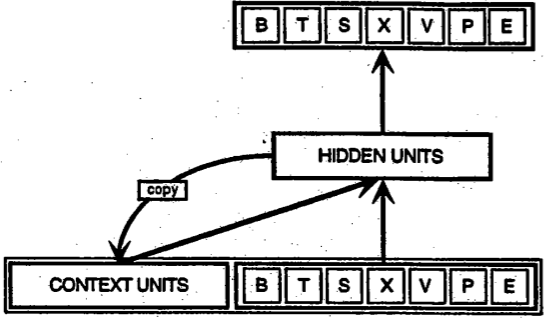
\includegraphics[width=7cm]{imgs/srn_net}\\
\end{center}

\subsection{Sieť s echo stavmi (ESN): architektúra, inicializácia, trénovanie modelu, vplyv parametrov na vlastnosti rezervoára, echo vlastnosť, pamäťová kapacita.}
Sieťe s echo stavmi sú typ rekurentnej neurónovej siete, ktorá má vstupnú vrstvu, rezervoár a výstupnú vrstvu.
Spojenia na vstupnej vrstve a v rekurentnej vrstve sa snažíme iba vhodne nainicializovat ale netrénujeme ich. To čo trénujeme je výstupná vrstva. Keďže sa teda snažíme trénovať len výstupnú vrstvu tak to vieme ľahko spraviť analyticky, čo je jednak rýchle a zároveň sa aj ľahko implementuje.\\
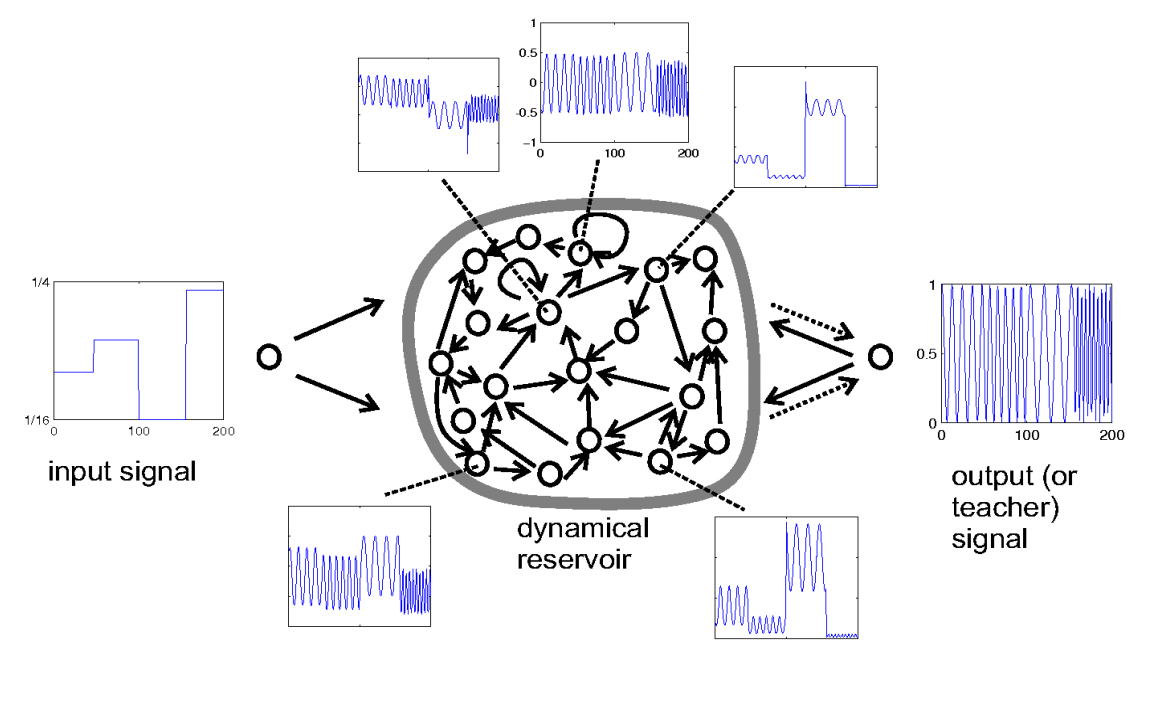
\includegraphics[width=10cm]{imgs/esn}\\
Na inicializáciu vstupných váh používame malé hodnoty z normálneho alebo rovnomerného rozdelenia. Rezervoár sa snažíme inicializovať tak, aby ma echo-state vlastnosť. \\
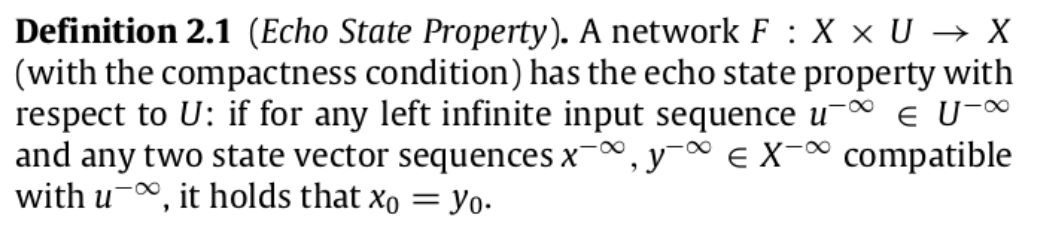
\includegraphics[width=10cm]{imgs/echo_prop}\\
Výstupnú vrstvu trénujeme pomocou pseudoinverznej matice $X$. 
Nech máme vstup $u_i$ a funkciu $f$, vzťahy pre prechod sieťou vyzerajú nasledovne: 
\begin{itemize}
\item $x(t) = f(W^{res}x(t-1) + W^{inp}u(t))$
\item $y(t) = f^{out}(W^{out}x(t))$
\end{itemize}
Kapacita pamäte prudko závisí od spektrálneho rádiusu, zvykne sa nastaviť zhruba na velkosť 0.9, ktorá ju optimalizuje. Spočítať ju môžeme takto:
$$MC = \sum_{k=1}^{k_{max}}MC_k = \sum_{k=1}^{k_{max}}\frac{cov^2(u(t-k),y_k(t)}{var(u(t)) var(y_k(t))}$$

\subsection{Hopfieldov model NS: deterministická dynamika, energia systému, relaxácia, typy atraktorov, autoasociatívna pamäť – nastavenie váh, princíp výpočtu kapacity pamäte.}

Hopfieldov model neurónovej siete vyzerá tak, že má jednu vrstvu, kde každý neurón je prepojený s ostatnými. Každý z neurónov nadobúda stav $S_i = \{-1,1\}, i = 1,\dots, n$ a má váhy $J_{ij}$. Ak $J_{ij} > 0$ nazývame ju excitačná inak inhibičná a definitoricky váha $J_{ii} = 0$. \\\\
V prípade, že chceme spočítať update váh najprv musíme spočítať:
\begin{enumerate}
\item Postsynaptický potenciál - $h_i^{int} = \sum J_{ij}S_j$.
\item Excitačná hranica(threshold) $h_i^{ext}$.
\item Efektívny postsynaptický potenciál $h_i = h_i^{int} - h_i^{ext}$.
\item Neuron state update(deterministic) $S_i \leftarrow sgn(h_i) \in \{-1,1\}$ ak $h_i=0$ potom $sgn(h_i) = 1$.
\end{enumerate}
Update môže prebiehať buď synchrónne(všetky naraz) alebo asynchróne(randomne po jednom). Je fajn si uvedomiť, že v prípade synchrónneho updatu sa hýbeme po vrcholoch hyperkocky ale v prípade asynchrónneho po jej hranách.
\\\\
 V každom stave siete vieme vypočítať takzvanú energiu siete $E = -\frac{1}{2}\sum_i\sum_jJ_{ij}S_iS_j - \sum_iS_ih_i^{ext}$
\\\\
Dá sa ukázať, že ak používame asynchrónny update s excitačným thresholdom $h_i^{ext} = 0, \forall i$ a symetrickou konektivitou neurónov $J = J^T$ energia vždycky klesá počas relaxácie(updatovania neurónov). 
\\\\
Atraktory delíme na pravé a falošné(lineárna kombinácia zapamätaných vzorov). 
\\\\
V autoasociatívnej pamäti chceme nastaviť váhy tak, aby bodovými atraktormi boli naše zapamätané patterny.
Predpokladajme, že máme binárne patterny $x{(p)} = [x_1^{(p)}, \dots, x_n^{(p)}]$ $p = 1, \dots, N$, potom váhy nastavíme podľa nasledovného vzťahu: 
$$ J_{ij} = \frac{1}{n}\sum_p x_i^{(p)} x_j^{(p)} \text{ for } i\neq j \text{ and } J_{ii} = 0$$
Keď sieť relaxujeme z $S(0) \to \dots \to x_i^{(r)}$ potom podmienka stability  pre vzor $x_i^{(r)}$ je nasledovná 
$$x_i^{(r)}\times h_i^{(r)} = x_i^{(r)}\sum_jJ_{ij}x_i^{(r)} = \dots = 1 + C_i^{(r)} > 0$$, 
kde $C_i^{(r)}$ voláme crosstalk(šum). Ak sú vzory na seba navzájom kolmé potom šum je $C_i^{(r)} = 0$ a kapacita pamäte je rovná počtu vzorov.
\\\\
Kapacitu pamäte môžeme merať pomocou toho, že zistíme aká je pravdepodobnosť, že $i$-ty neurón je nestabilný. $P_{error} = P(C_i^{(r)} > 1)$. Táto pravdepodobnosť priamo závisí od počtu patternov a počtu neurónov. $C_i^{(r)} \sim Bin(0,\sigma^2)$ kde $\sigma^2 = N/n$. Z vety o centrálnej limite potom platí, že $Bin\approx N(0, \sigma^2)$.


\subsection{Nelineárne dynamické systémy: stavový portrét, dynamika, typy atraktorov. Hopfieldov model NS: stochastická dynamika, parameter inverznej teploty, princíp odstránenia falošných atraktorov.}
\textcolor{red}{TODO}


\end{document}